\chapter{Software Design, Implementation and Testing}
\label{software}
%TC:ignore
\begin{comment}
This could be one chapter or a few chapters. It should define and discuss the software that is developed to support the research that is being conducted. For example, if your research involves running experiments, what software are you creating to support that work? What functionality is required? What design will be used? What implementation issues are there and what testing is used? 

Even though a research project is investigating specific research questions, it is still necessary for you to discuss the software that you develop. Research has a habit of generating bits of software that can exist for several years and need future modification. Therefore you need to be able to discuss the technical issues as well as the research approach. 
\end{comment}
%TC:endignore


\section{Design}
%TC:ignore
\begin{comment}
You should concentrate on the more important aspects of the design. It is essential that an overview is presented before going into detail. As well as describing the design adopted it must also explain what other designs were considered and why they were rejected.

The design should describe what you expected to do, and might also explain areas that you had to revise after some investigation.

Typically, for an object-oriented design, the discussion will focus on the choice of objects and classes and the allocation of methods to classes. The use made of reusable components should be described and their source referenced. Particularly important decisions concerning data structures usually affect the architecture of a system and so should be described here.

How much material you include on detailed design and implementation will depend very much on the nature of the project. It should not be padded out. Think about the significant aspects of your system. For example, describe the design of the user interface if it is a critical aspect of your system, or provide detail about methods and data structures that are not trivial. Do not spend time on long lists of trivial items and repetitive descriptions. If in doubt about what is appropriate, speak to your supervisor.
 
You should also identify any support tools that you used. You should discuss your choice of implementation tools - programming language, compilers, database management system, program development environment, etc.

Some example sub-sections may be as follows, but the specific sections are for you to define. 
\end{comment}
%TC:endignore
\subsection{Overall Architecture}

python modules, object oriented:

ImageManager to handle loading, saving and standardising images and running the methods. Discussed in detail in section \ref{ImageManger}

flask server to run UI and call ImageManager in user friendly way. Discussed in detail in section \ref{FlaskServer}

finders, classes to implement the methods, flexible

\begin{figure}
    \centering
    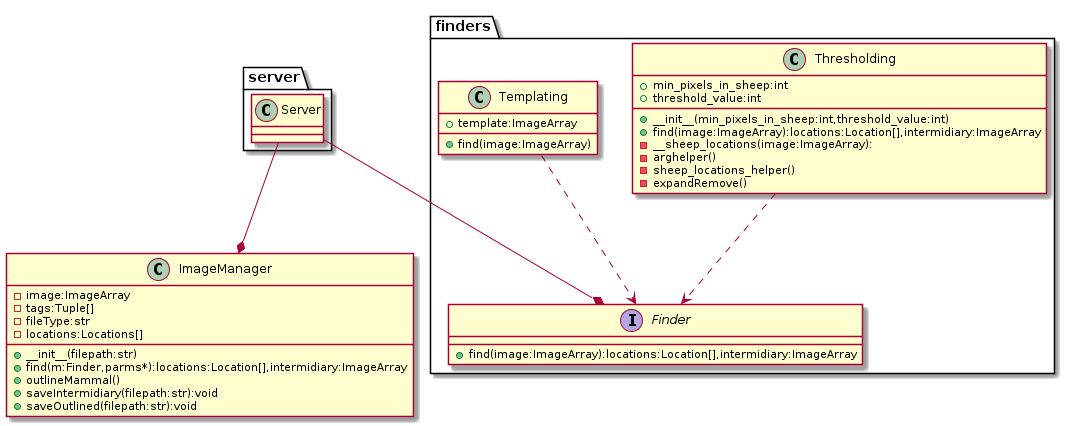
\includegraphics[width=\textwidth]{diagrams/uml.png}
    \caption{UML Class Diagram}
    \label{fig:uml}
\end{figure}

\subsection{Image Manager}
\label{ImageManger}

\subsubsection{Even more detail}

\subsection{User Interface}
\label{FlaskServer}

\subsection{Finders}
\subsubsection{Templating}
\subsubsection{thresholding}

\section{Implementation}

%TC:ignore
\begin{comment}
This section should discuss issues you encountered as you tried to implement your experiments. What were the results of running the experiments? What conclusions can you draw from these results? 

During the work, you might have found that elements of your experiments were unnecessary or overly complex; perhaps third-party libraries were available that simplified some of the functions that you intended to implement. If things were easier in some areas, then how did you adapt your project to take account of your findings?

It is more likely that things were more complex than you first thought. In particular, were there any problems or difficulties that you found during implementation that you had to address? Did such problems simply delay you or were they more significant? 

If you had multiple experiments to run, it may be sensible to discuss each experiment in separate sections. 
\end{comment}
%TC:endignore

\section{Testing}
%TC:ignore
\begin{comment}
Detailed descriptions of every test case are definitely not what is required in this section; the place for detailed lists of tests cases is in an appendix. In this section, it is more important to show that you adopted a sensible strategy that was, in principle, capable of testing the system adequately even if you did not have the time to test the system fully. 

Provide information in the body of your report and the appendix to explain the testing that has been performed. How does this testing address the requirements and design for the project?

How comprehensive is the testing within the constraints of the project?  Are you testing the normal working behaviour? Are you testing the exceptional behaviour, e.g. error conditions? Are you testing security issues if they are relevant for your project?

Have you tested your system on ``real users''? For example, if your system is supposed to solve a problem for a business, then it would be appropriate to present your approach to involve the users in the testing process and to record the results that you obtained. Depending on the level of detail, it is likely that you would put any detailed results in an appendix. 

Whilst testing with ``real users'' can be useful, don't see it as a way to shortcut detailed testing of your own. Think about issues discussed in the lectures about until testing, integration testing, etc. User testing without sensible testing of your own is not a useful activity.

The following sections indicate some areas you might include. Other sections may be more appropriate to your project. 
\end{comment}
%TC:endignore

\subsection{Overall Approach to Testing}

Do little and often, while developing, write tests as I go, does this do what I want it to?

\subsection{Automated Testing}
Using an automated testing system such as Jenkins was considered but as the code for this project only produces images,  setting up a system to test them automatically would be a hassle as the code is not expected to produce perfect identical results every time and once the system to load and save the images is created it will not require ongoing testing. Unit testing that will be manually run will be created for testing that part. To produce the results the code behind that will be simple scripts that will be manually run.

\subsubsection{Unit Tests}

done some of this but very little

\subsubsection{User Interface Testing}

not done this..

\subsubsection{Stress Testing}

Use biggest image I have available, with most complex set of parameters.

\subsection{Integration Testing}

\subsection{User Testing}
